\documentclass[aspectratio=1610]{beamer}
\setbeamertemplate{frametitle continuation}[from second][(contd.)]
\title{Changing Norms and Partisan Polarization: How elites advance mass polarization}
\subtitle{Prepared for presentation in a seminar of Political Psychology}
\date{\today}
\author[\copyright\ Roberts $2021$]{Damon C. Roberts, University of Colorado}

\input{/Users/damonroberts/Dropbox/personal/beamer_template/preamble.tex}

\begin{document}
	\begin{frame}
		\maketitle	
	\end{frame}
	\begin{frame}
		\frametitle{How we think of polarization}
		\begin{itemize}
			\item Polarization as the result of divergent issue preferences
			\item Polarization as the result of social identities
		\end{itemize}
	\end{frame}
	\begin{frame}[allowframebreaks]
		\frametitle{What I argue}
		\begin{itemize}
			\item Agrees that polarization is likely the result of divergent and converging (as opposed to cross-cutting) identities
			\item In the world of a low information Jordan Q. Public, behavioral manifestations should be coming from somewhere
			\item It is coming from norms
			\begin{itemize}
				\item Elites are polarized both ideologically and affectively (Enders 2021)
				\item Elites have significant influence in the formation of attitudes among the public (Zaller 1992) and of partisans (Layman and Carsey 2002)
				\item The mass media are a common link between voters and politicians
				\item The mass media often interpret political events and the behaviors of actors
				\item This information helps teach the public about what behaviors are normal and the extent to which they are so
				\item As good partisans, the public then pick these behaviors up
				\item As a set of group norms, partisans will evaluate co-partisans and out-partisans based on how they adopt these norms as well.
			\end{itemize}
		\end{itemize}
	\end{frame}
	\begin{frame}
		\frametitle{Study 1}
		\begin{itemize}
			\item Examine predictors of polarization and of behavioral manifestations of polarization over time. In particular, in line with my hypotheses, look at campaign attention and media consumption. 
			\item ANES with its consistency* over time
		\end{itemize}
	\end{frame}
	\begin{frame}
		\frametitle{Study 2}
		\begin{itemize}
			\item Field survey of open ended responses with the goal of getting a sense of what behaviors the public think are normal in relation to politics and to see if there is partisan heterogeneity
			\item Prime them to think about group differences through a Party Likes/Dislikes exercise
			\item Use two questions:
			\begin{itemize}
				\item ``What does it look like to be a \textbf{Republican/Democrat}?"
				\item ``Please describe what is the right way to talk to \textbf{Democrats/Republicans}"
			\end{itemize}
			\item Plan of analysis
			\begin{itemize}
				\item Either Unsupervised approaches like Topic Modeling, or do a supervised approach with some human coders. Or both!
			\end{itemize}
		\end{itemize}
	\end{frame}
	\begin{frame}
		\frametitle{Study 3}
		\begin{itemize}
			\item Use information culled from Study 2 to do an experiment
		\end{itemize}
		\begin{table}[hbt!]
			\caption{2x3 Factorial Design}
			\begin{tabular}{p{0.2\linewidth}p{0.2\linewidth}p{0.2\linewidth}p{0.2\linewidth}p{0.2\linewidth}}
				\textbf{} & \textbf{Co-Partisan} & \textbf{Out-Partisan} & \textbf{No Interpretation}\\
				\midrule
				\textit{Republican} & Republican \& Republican elite & Republican \& Democrat elite & Republican \& No Interpretation \\ [1ex]
				\\
				\hdashline 
				\\ 
				\textit{Democrat} & Democrat \& Democratic elite & Democrat \& Republican elite & Democrat \& No Interpretation \\
				\hline
			\end{tabular}
		\end{table}\textbf{}
	\end{frame}
	\begin{frame}[allowframebreaks]
		\frametitle{Example of Vignette for Republican Participants}
	Congress introduced a new bill today. The bill \textbf{disliked by Republicans} is meant to address funding concerns for high use interstate highways. In reference to the bill, \textbf{Republican Leadership} expressed their feelings indicating that they felt this bill was not important. During the floor vote \textbf{Republicans spoke at length about the Democrats' desire to slow Congress down with "pointless bills"}. Afterwards on the floor, \textbf{Republicans were huddled talking about how to make sure it doesn't come back up for a vote next session}. That afternoon, when speaking to the press, \textbf{Republican leaders talked about how Democrats don't care about the well-being of the country}.
	\end{frame}
	\begin{frame}[allowframebreaks]
		\frametitle{Example of Vignette for Placebo}
		Congress introduced a new bill today. The bill \textbf{supported by Republicans} is meant to address funding concerns for high use interstate highways. In reference to the bill, \textbf{Republican Leadership} expressed their feelings indicating that they felt this bill was not important. During the floor vote \textbf{Republicans spoke at length about how there are more important things to consider on the agenda}. Afterwards on the floor, \textbf{members were seen running off to their next committee meeting}. That afternoon, when speaking to the press, \textbf{Republican leaders expressed frustration but is hopeful for future negotiations to go their way.}
	\end{frame}
	\begin{frame}
		\frametitle{Measuring Polarization}
		\begin{itemize}
			\item Standard Feeling Thermometer questions of each party: FT of In-group - FT of Out-group
			\item ``Do you think the Republican leadership's response was appropriate?"
			\item ``Should the Democrats have reacted the way they did on the floor by getting in a huddle?"
		\end{itemize}
	\end{frame}
	\begin{frame}
		\frametitle{Power analysis}
		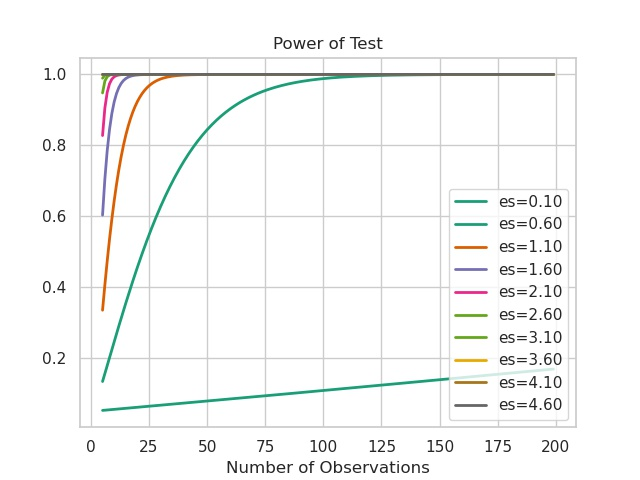
\includegraphics[width = 100mm]{../figures/power_analysis}	
	\end{frame}

	\begin{frame}
		\frametitle{Feedback}
		Replication code for power analysis: 
		
		
\includegraphics[width = 50mm]{qr_code}
	\end{frame}
\end{document}